\documentclass{beamer}

\usetheme{Goettingen}

%\usepackage{beamerthemesplit}
\usepackage{ucs}
\usepackage[utf8x]{inputenc}
\usepackage{ngerman}
\usepackage{graphicx}
\usepackage{tabularx}

\setbeamertemplate{footline}[frame number]

\begin{document}

\title[Hickerspace]{Hickerspace, der Hackerspace in Hildesheim}
\subtitle{Aktueller Stand}
\author[]{}
\date{29.11.2013}

%-----------------------------------------------------

\frame{\titlepage} 

%-----------------------------------------------------

\frame{\frametitle{Übersicht}\tableofcontents} 

%-----------------------------------------------------

\section{Hickerspace}

\subsection{Allgemeines}

\frame{\frametitle{Einleitung: Allgemeines} 
\begin{itemize}
\item Existenz seit Mitte 2008
\item Entscheidung damals: keine Mitgliedschaften, keine Beiträge
\item Regelmäßige Treffen Freitags ab 20 Uhr, bei Bedarf Zusatzzermine
\item Anschaffungen durch Getränkeverkauf und Crowd-Funding
\item Grundprinzip: Konsens-Entscheidungen
\end{itemize}}

\subsection{Themengebiete}

\frame{\frametitle{Themengebiete} 
\begin{itemize}
\item Individuelle und gemeinsame Projekte (Hardware, Software, Food-Hacking)
\item Wissensaustausch und -vermittlung
\item Vorträge, Workshops
\item Kochen
\item Netzpolitisches
\end{itemize}}

\subsection{Projektwerkstatt}

\frame{\frametitle{Derzeitiger Raum: Projektwerkstatt} 

\begin{itemize}
\item Büroraum in der Kulturfabrik Löseke (ca. 36 Quadratmeter)

\item Finanziert durch die Stadt Hildesheim
\item Regelmäßige Treffen unterschiedlicher Gruppen
    \begin{itemize}
    \item Zeit und Raum pro Gruppe begrenzt
    \end{itemize}
\item Grundlegende technische Infrastruktur vorhanden
\end{itemize}}


\section{Projekte}

\frame{\frametitle{Projekte} 
\begin{itemize}
\item Eine kleine Auswahl bisher abgeschlossener Projekte.
\end{itemize}
}


\subsection{Hardware}

\frame{\frametitle[width=0.4\textwidth]{Hardware: Mousemodding (1. Projekt)} 

\begin{figure}[]
    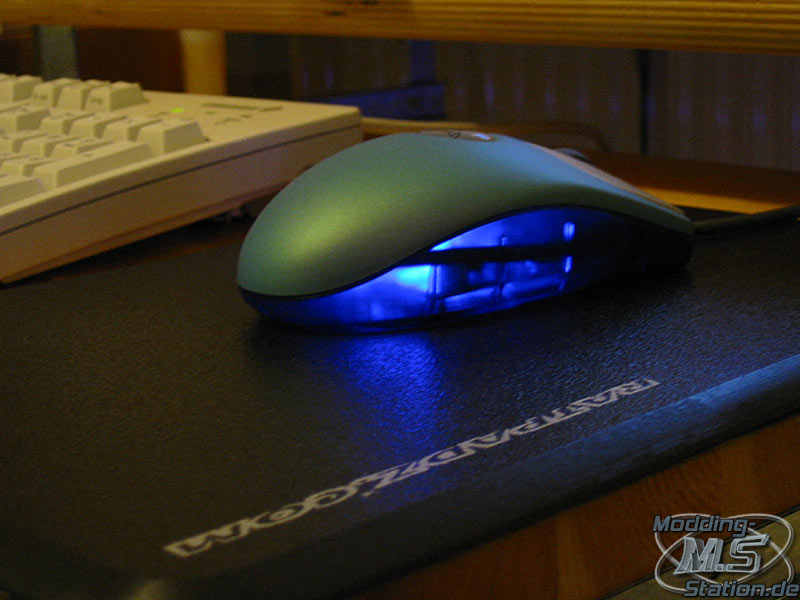
\includegraphics[height=6cm]{figures/maus.png}
\end{figure}

}

\frame{\frametitle[width=0.4\textwidth]{Hardware: Die Seifenblasenmaschine} 

\begin{figure}[]
    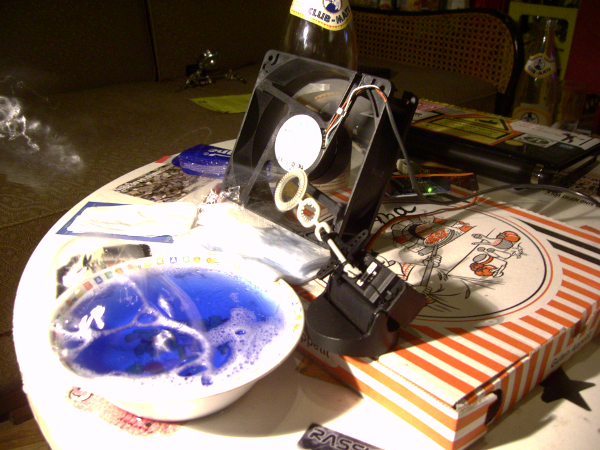
\includegraphics[height=6cm]{figures/seifenblasen.png}
\end{figure}

}

\frame{\frametitle{Ampel} 

\begin{figure}[]
    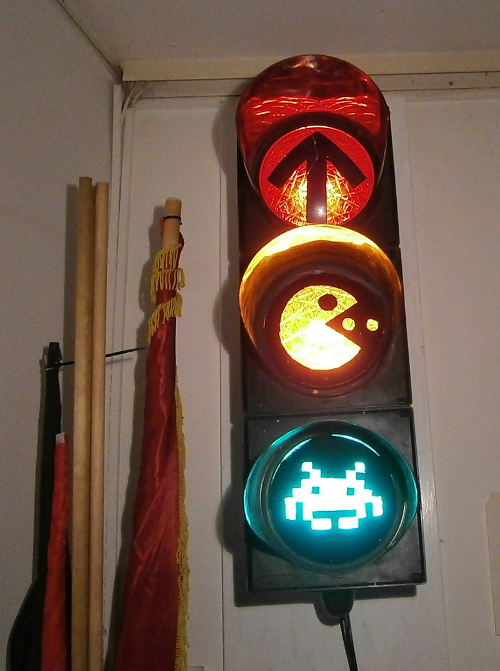
\includegraphics[height=6cm]{figures/ampel.png}
\end{figure}

}

\frame{\frametitle{Hardware: Neuland-Ortsschild} 

\begin{figure}[]
    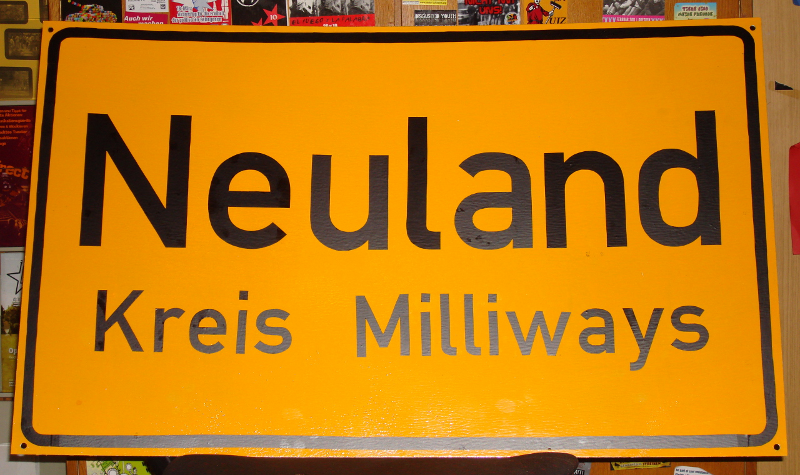
\includegraphics[height=6cm]{figures/neuland.png}
\end{figure}

}

\subsection{Software}

\frame{\frametitle{Software: Microprinting} 

\begin{figure}[]
    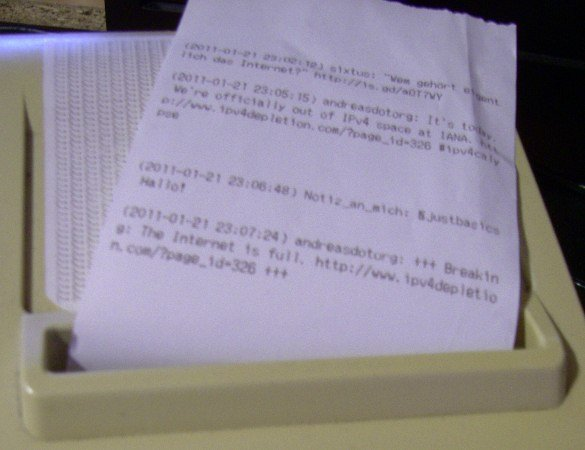
\includegraphics[height=6cm]{figures/bon.png}
\end{figure}

}

\frame{\frametitle{Software: LED-Bahnanzeige} 

\begin{figure}[]
    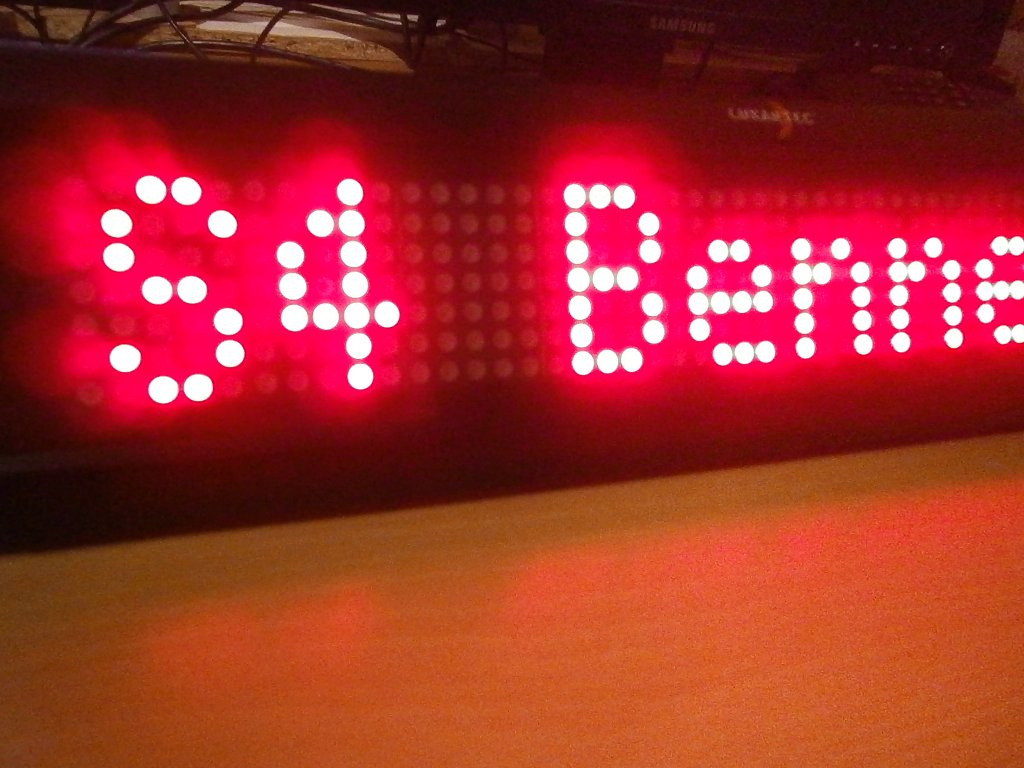
\includegraphics[height=6cm]{figures/ben.png}
\end{figure}

}

\subsection{Food-Hacking}

\frame{\frametitle{Food: Matelade} 

\begin{figure}[]
    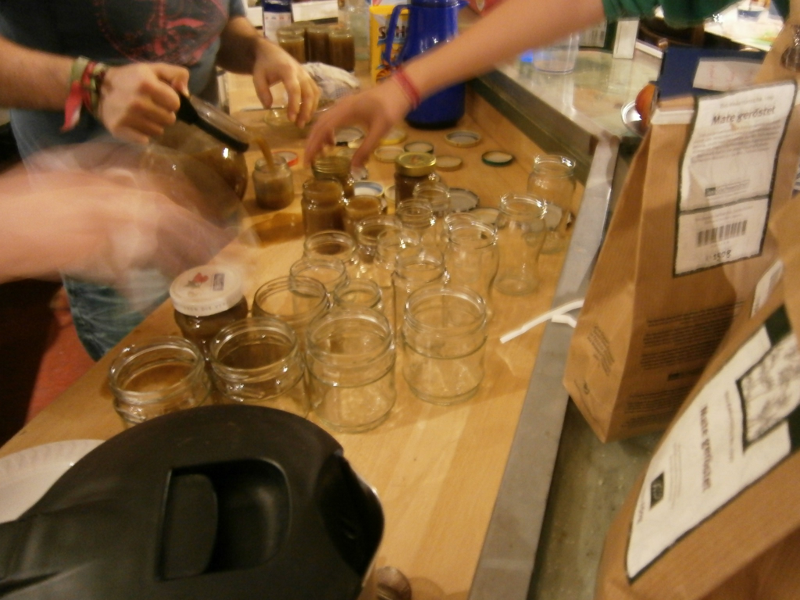
\includegraphics[height=6cm]{figures/matelade.png}
\end{figure}

}

\frame{\frametitle{Food: Pizza} 

\begin{figure}[]
    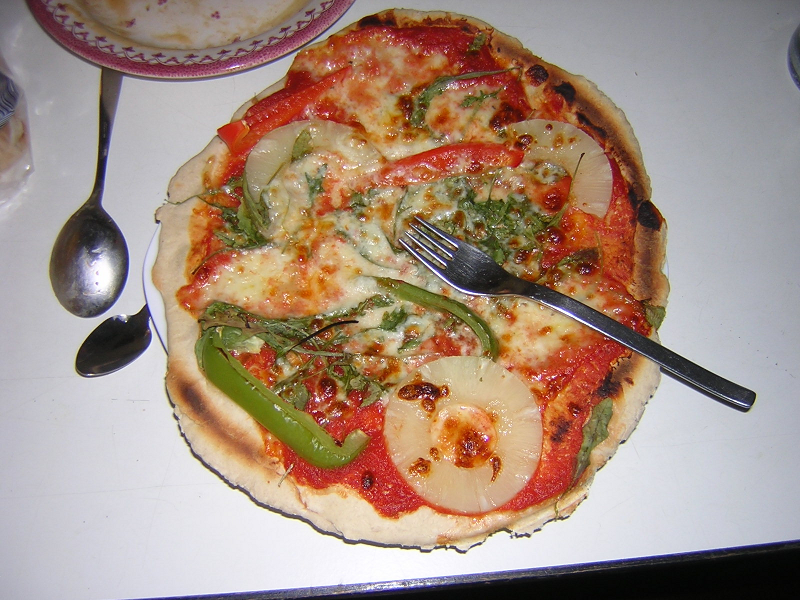
\includegraphics[height=6cm]{figures/pizza.png}
\end{figure}

}

\frame{\frametitle{Food: Pizza-Soße (eine Woche später)} 

\begin{figure}[]
    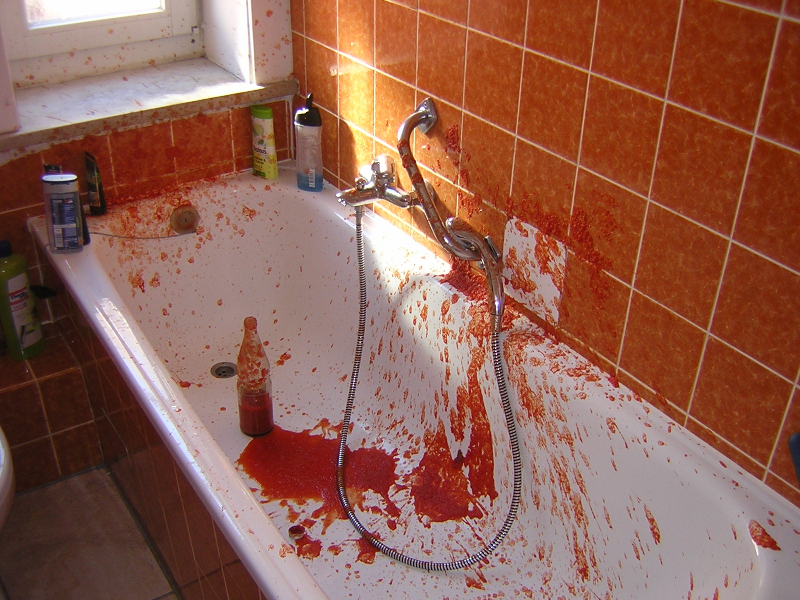
\includegraphics[height=6cm]{figures/sosse.png}
\end{figure}

}



\frame{\titlepage} 



\end{document}
